%!TEX root = draft.tex

\section{Motivating Example}

\begin{figure*}[t]
\lstset{numbers=left, 
            numberstyle=\tiny\tt, 
            stepnumber=1, 
            firstnumber=1,
            % numberfirstline=true,
            numbersep=4pt}
\begin{minipage}{5cm}
\begin{program}
struct node {
	int data;
	struct node *next;
}
struct stack {
	struct node *Top
}
  
struct stack *S;
\end{program}
\end{minipage}
\begin{minipage}{6.5cm}
{\bf Lock-based stack:}
\begin{program}
void push(int v) {
	lock();
	struct node *n;
	n = malloc(sizeof( *x));
	n->data = v;
	n->next = S->Top;
	S->Top = n;
	unlock();
}

\end{program}
\end{minipage}
\begin{minipage}{6cm}
{\bf Treiber's stack:}
\begin{program}
void push(int v) {
	struct node *n,*t;
	n = malloc(sizeof( *n));
	n->data = v;
	do {
		struct node *t = S->Top;
		n->next = t;
	} while (! CAS (&S->Top, t, n))
}
\end{program}
\end{minipage}

%{\bf Treiber's stack:}
\begin{minipage}{5cm}
\lstset{numbers=none}
{\bf Client program $P$:}

\begin{minipage}{1.8cm}
%\begin{center}
%{\bf Thread 1}
%\end{center}
\bigskip
{\bf Thread1:}
\vspace{-1mm}
%$\mbox{\bf Thread 1:}$
\begin{program}
push(1);
x = pop();
y = pop();
\end{program}
\end{minipage}
\begin{minipage}{.5cm}
%\hspace{1mm}
\vspace{6mm}
{\large $\bigparallel$}
%\hspace{2mm}
\end{minipage}
\begin{minipage}{2cm}
\bigskip
{\bf Thread2:}
\vspace{-1mm}
\begin{program}
z = pop();
push(2);
push(3);
\end{program}
\end{minipage}
\end{minipage}
\begin{minipage}{6.5cm}
\lstset{firstnumber=10}
\begin{program}
int pop() {
	lock()
	struct node *t = S->Top;
	if (t==NULL)
		return EMPTY;
	S->Top = t->next;
	unlock()
	return t-> data;
}
\end{program}
\end{minipage}
\begin{minipage}{6cm}
\lstset{firstnumber=10}
\begin{program}
int pop() {
	struct node *n,*t;
	do {
		*t = S->Top;
		if (t==NULL)
			return EMPTY;
		n = t->next;
	} while (! CAS (&S->Top, t, n))
	int result = t->data;
	free(t);
	return result;
}

\end{program}
\end{minipage}

{\footnotesize
\hspace{.2cm}
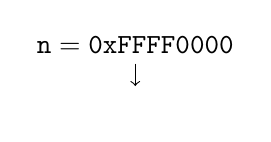
\begin{tikzpicture}[node distance=.7cm]
\tikzstyle{node}=[minimum size=10pt]
\node[node] (x)  [] at (1, 0) {${\tt n} = {\tt 0xFFFF 0000}$};
\node[node] (y)  [below of=x] {}; %label=above:$x$
\draw[->] (x) -- (y); %node[draw=none,right] {$h$}
\end{tikzpicture}
\hspace{0.7cm}
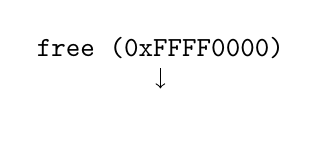
\begin{tikzpicture}[node distance=.7cm]
\tikzstyle{node}=[minimum size=10pt]
\node[node] (x)  [] at (1, 0) {{\tt free (0xFFFF0000)}};
\node[node] (y)  [below of=x] {}; %label=above:$x$
\draw[->] (x) -- (y); %node[draw=none,right] {$h$}
\end{tikzpicture}
\hspace{2.8cm}
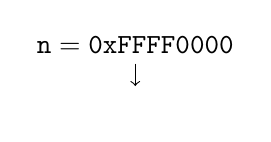
\begin{tikzpicture}[node distance=.7cm]
\tikzstyle{node}=[minimum size=10pt]
\node[node] (x)  [] at (1, 0) {${\tt n} = {\tt 0xFFFF 0000}$};
\node[node] (y)  [below of=x] {}; %label=above:$x$
\draw[->] (x) -- (y); %node[draw=none,right] {$h$}
\end{tikzpicture}

\vspace{-1cm}
\[
\underbrace{\<push>(1)_1\ldots \<ret>_1\ \<pop>_2\ldots ^{8}}_{\tt {\bf Thread 1}} \ddagger\
\underbrace{\<pop>()_3\ldots \<ret>(1)_3\ z=1\ \<push>(2)_4\ldots \<ret>_4\ \<push>(3)_5\ldots \<ret>_5}_{\tt {\bf Thread 2}} \ddagger\ 
\underbrace{^{8}\ldots  \<ret>(3)_2\ x=3\ \<pop>()_6\ldots \<ret>({\tt EMPTY})_6\ y={\tt EMPTY}}_{\tt {\bf Thread 1}}
\]
}
\caption{A reference lock-based implementation of a concurrent stack and Treiber's stack implementation ({\tt EMPTY} is a special value denoting the empty stack). The client program $P$ consists of two concurrent threads executing the statements in the left and respectively, the right of the $\parallel$ symbol.}
\label{fig:stacks}
\end{figure*}

Figure~\ref{fig:stacks} contains a reference lock-based implementation for a concurrent stack and an implementation of the non-blocking Treiber's stack~\cite{Treiber'86}. Both implementations represent the stack using a singly-linked list rooted at {\tt S->Top}. The methods of the reference implementation execute all statements in one atomic step while in Treiber's stack, methods execute non-atomically and their statements may interleave. The variable {\tt S->Top} of Treiber's stack is updated using the primitive {\tt CAS} (compare-and-swap), which assigns {\tt x} to {\tt S->Top} only if its current value equals the second argument {\tt t} (the equality test and the assignment are performed in one atomic step).

The implementation of Treiber's stack is more efficient because it minimizes the synchronization overhead when updating the stack. However, it is known that this implementation does not conform to the reference stack implementation (based on locks) because it suffers from the infamous ABA bug due to freeing popped nodes.

A classic formalization of conformance to reference implementations is called \emph{observational refinement}. Essentially, an implementation $L_1$ is an observational refinement of another implementation $L_2$ if every observable behavior of a client program $P$ using $L_1$ is also possible when $P$ uses $L_2$. For example, Treiber's stack is not an observational refinement of the lock-based implementation because the program $P$ given in Figure~\ref{fig:stacks} can reach a state where $x=3$ and $y={\tt EMPTY}$ when using Treiber's stack but not when using the lock-based implementation. Intuitively, reaching this state corresponds to an incorrect behavior of the stack: when popping $3$ from the stack, the latter should still contain the value $2$ (it shouldn't be empty). 

The execution of $P$ when using Treiber's stack, that reaches $x=3$ and $y={\tt EMPTY}$, is given in the bottom of Figure~\ref{fig:stacks}. Thus, {\bf {\tt Thread1}} starts executing and it is preempted when reaching line 8 of the second call to $\<pop>$. Then, {\bf {\tt Thread2}} executes until completion followed by {\bf {\tt Thread1}}. Furthermore, the {\tt malloc} from the last $\<push>$ in {\bf {\tt Thread2}} returns the same address that was freed in the first $\<pop>$ from {\bf {\tt Thread1}}. The local state of the pending $\<pop>$ when {\bf {\tt Thread1}} is preempted contains ${\tt t}={\tt 0xFFFF0000}$ and ${\tt n}={\tt NULL}$. Since the address ${\tt 0xFFFF 0000}$ is reused in the last $\<push>$ from {\bf {\tt Thread2}}, the value of {\tt S->top} when {\bf {\tt Thread1}} resumes equals {\tt 0xFFFF0000}. Therefore, the {\tt CAS} executed by {\bf {\tt Thread1}} will succeed and {\tt S->top} becomes {\tt NULL}. The element $2$ pushed by {\bf {\tt Thread2}} is lost and the last $\<pop>$ from  {\bf {\tt Thread1}} returns {\tt EMPTY}. Note that this behavior is not possible when $P$ uses the reference implementation where methods execute in one atomic step.












